\section{ 心を開いて}

\large{

\ruby{私}{わたし}はあなたが\ruby{想}{おも}ってる\ruby{様}{よう}な\ruby{人}{ひと}では

ないかもしれない

でも\ruby{不思議}{ふしぎ}なんだけど

あなたの\ruby{声}{こえ}を\ruby{聞}{き}いてると

とても \ruby{優}{やさ}しい\ruby{気持}{きも}ちになるのよ
\\

このままずっと \ruby{忘}{わす}れたくない

\ruby{現実}{いま}が\ruby{想}{おも}い\ruby{出}{で}に\ruby{変}{か}わっても

\ruby{言葉}{ことば}はないけど きっとあなたも

\ruby{同}{おな}じ\ruby{気持}{きも}ちでいるよね
\\

\parpic[r]{
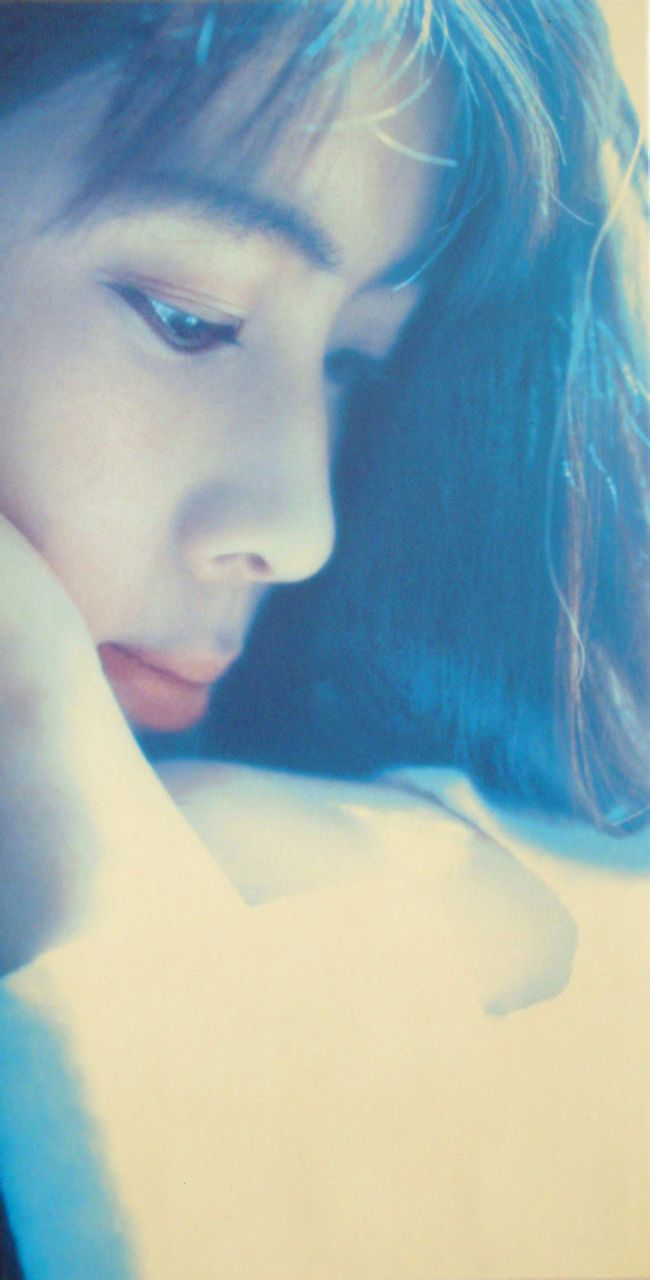
\includegraphics[width=0.3\textwidth]{S18.jpg}}

\ruby{人}{ひと}と\ruby{深}{ふか}くつきあうこと

\ruby{私}{わたし}もそんなに\ruby{得意}{とくい}じゃなかった

でも あなたを\ruby{見}{み}ていると

\ruby{私}{わたし}と\ruby{似}{に}ていて もどかしい

そういう\ruby{所}{ところ}が たまらなく\ruby{好}{す}きなの
\\

ビルの\ruby{隙間}{すきま}に\ruby{二人}{ふたり}\ruby{座}{すわ}って

\ruby{道}{みち}\ruby{行}{い}く\ruby{人}{ひと}を ただ\ruby{眺}{なが}めていた

\ruby{時間}{ときかん}が\ruby{過}{す}ぎるのが \ruby{悲}{かな}しくて

あなたの\ruby{肩}{かた}に\ruby{寄}{よ}りそった
\\

My dream Your smile

\ruby{忘}{わす}れようとすればする\ruby{程}{ほど} \ruby{好}{す}きになる

それが\ruby{誤解}{ごかい}や\ruby{錯覚}{さっかく}でも…

\ruby{心}{こころ}を\ruby{開}{ひら}いて
\\

どんなときも あなたの\ruby{胸}{むね}に

\ruby{迷}{まよ}わず\ruby{飛}{と}び\ruby{込}{こ}んでゆくわ

Your dream I believe

ときめいてる \ruby{心}{こころ}を\ruby{開}{ひら}いて

}